\documentclass[11pt,a4paper]{ctexart}

\usepackage[margin=2.6cm]{geometry}
\usepackage{amsmath,amssymb,amsthm}
\usepackage{graphicx}
\usepackage{booktabs}
\usepackage{hyperref}
\usepackage{xcolor}
\usepackage{listings}
\usepackage{caption}

\graphicspath{{figures/}}
\hypersetup{colorlinks=true, linkcolor=blue!50!black, urlcolor=blue!60!black}
\lstset{
  basicstyle=\ttfamily\small,
  breaklines=true,
  frame=single,
  columns=fullflexible,
  backgroundcolor=\color{gray!7}
}

\title{时间序列中的趋势 \\ \large Trends in a time series}
\author{基于 \textit{A Course in Time Series Analysis} 的中文讲义与 Python 实践}
\date{}

\begin{document}
\maketitle

\section*{本章定位}

本章对应原文 \textit{Trends in a time series}。首版讲义先按照原文的章节主线整理核心概念、教学解释和 Python 工程实践；后续精修时，可继续把原 PDF 中的证明、练习和细节推导逐节扩展进来。

本章范围：趋势估计、差分、非参数平滑、周期函数和周期检测。

\section{核心知识点}

\begin{itemize}
  \item 参数趋势可用最小二乘估计，但残差相关会影响标准误。
  \item 差分用于削弱低频趋势，使序列更接近平稳。
  \item 移动窗口、筛估计和傅里叶工具把趋势与周期放在统一框架中。
\end{itemize}

\section{教学说明}

学习本章时，建议先区分三个层次：第一，模型或概念试图刻画哪一种时间序列现象；第二，对应的数学对象是什么，例如均值函数、自协方差函数、谱密度或条件方差；第三，在 Python 中如何通过仿真、估计和图形诊断把抽象概念落到可观察对象上。

对于原文中的 R 代码，本项目统一改写为 Python。常用工具包括 \texttt{numpy}、\texttt{pandas}、\texttt{matplotlib}、\texttt{scipy} 和 \texttt{statsmodels}。这些库覆盖了数据组织、数值计算、图形生成、频域分析、ARMA 仿真和 ACF/PACF 诊断。

\section{Python 工程实践}

在本章目录下运行：

\begin{lstlisting}[language=bash]
python scripts/ch02_generate_figures.py
\end{lstlisting}

脚本会把图像写入本章 \texttt{figures/} 目录。图像既可用于教学解释，也可作为后续扩充案例的基础。

\begin{figure}[htbp]
  \centering
  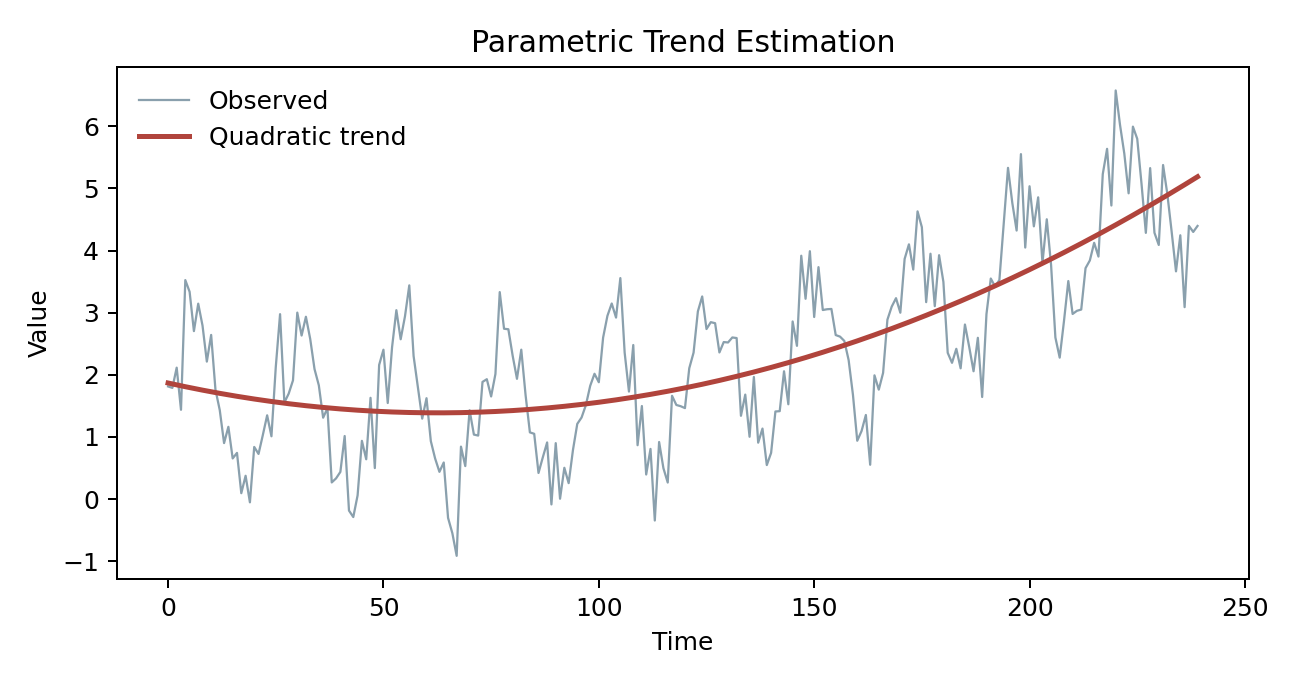
\includegraphics[width=0.86\textwidth]{ch02_fig01_parametric_trend.png}
  \caption{时间序列中的趋势 Python 实践图：ch02\_fig01\_parametric\_trend.png}
\end{figure}

\begin{figure}[htbp]
  \centering
  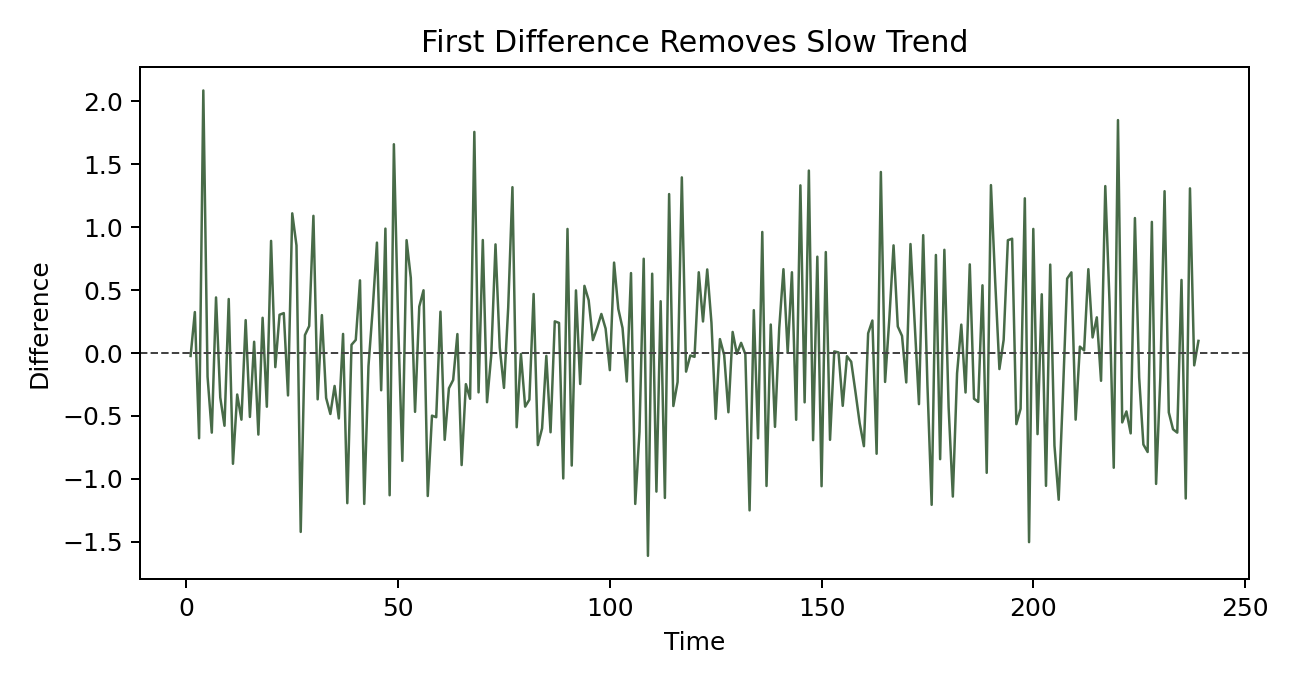
\includegraphics[width=0.86\textwidth]{ch02_fig02_differencing.png}
  \caption{时间序列中的趋势 Python 实践图：ch02\_fig02\_differencing.png}
\end{figure}

\begin{figure}[htbp]
  \centering
  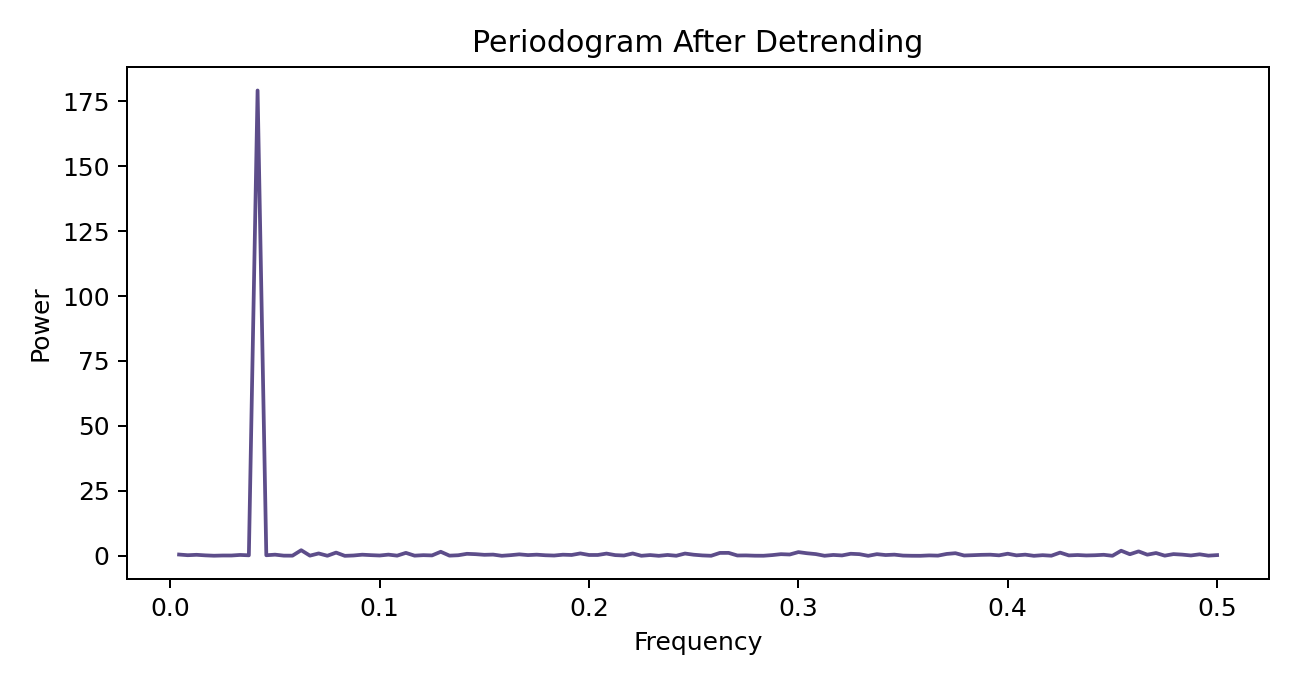
\includegraphics[width=0.86\textwidth]{ch02_fig03_periodogram.png}
  \caption{时间序列中的趋势 Python 实践图：ch02\_fig03\_periodogram.png}
\end{figure}

\section{本章小结}

本章首版的重点是建立概念地图和可运行实践。后续精修建议按原文小节逐段扩展：先补齐定义和定理，再补证明思路，最后增加练习题解析和真实数据案例。

\end{document}
